\section{MUMPS: Process Pinning}
\label{subseq:mm-mumps-process-pinning}

Due to intensive and complex manipulations with frontal and and contribution matrices, we can assume that MUMPS belongs to memory bound applications. In this case memory access can be a bottleneck for the library. A common way to improve performance of memory bound applications running on distributed memory machines is to distribute processes equally among sockets of a node.\\


However, because MUMPS uses both task and data parallelism as well as a complex hybrid, both static and dynamic, task scheduling, it becomes difficult to decide which pinning strategy is better i.e. \textit{close} or \textit{spread}, described in section \ref{subseq:matrix-sets-and-hardware}.\\


Therefore, a couple of tests were conducted with both GRS and SuiteSparse matrix sets in order to investigate which strategy worked better in terms of parallel performance. For this group of tests, we used only MUMPS default settings. The tests were performed on HW1 machine using only flat-MPI mode. Some results are shown in figure \ref{fig:mumps-close-vs-spread} and in appendix BRA-BRA. During the tests, the total time spent, i.e. analysis, factorization and solution, was measured.\\


\figpointer{\ref{fig:mumps-close-vs-spread}}
\begin{figure}[htpb]
\centering
	\begin{tabular}{cc}
		\subfloat[cube-5]{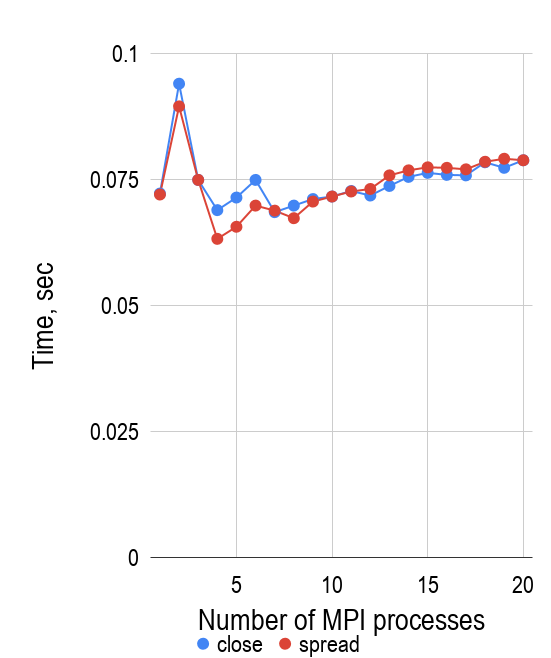
\includegraphics[width=0.48\textwidth]{figures/chapter-2/spread-vs-close/cube-5.png}} &
		\subfloat[pwr-3d]{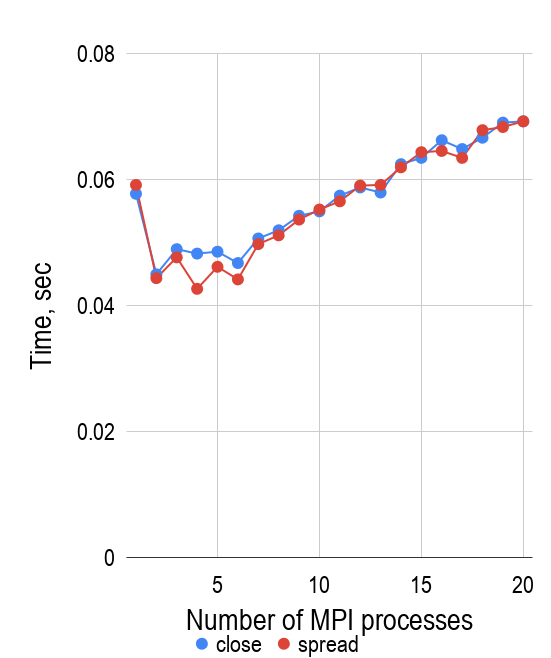
\includegraphics[width=0.48\textwidth]{figures/chapter-2/spread-vs-close/pwr-3d.png}} \\
		\subfloat[k3-2]{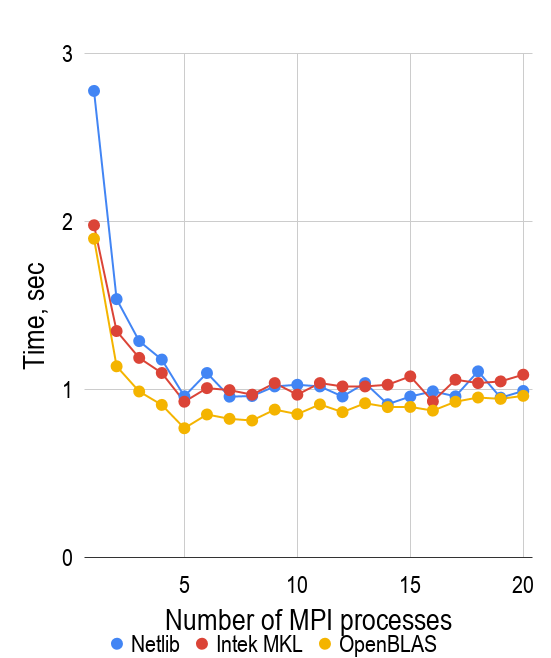
\includegraphics[width=0.48\textwidth]{figures/chapter-2/spread-vs-close/k3-2.png}} &
		\subfloat[k3-18]{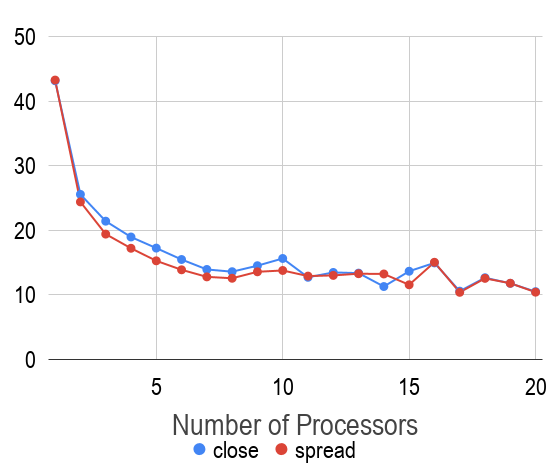
\includegraphics[width=0.48\textwidth]{figures/chapter-2/spread-vs-close/k3-18.png}} \\
	\end{tabular}
	\caption{Comparison of \textit{close} and \textit{spread} pinning strategies}
	\label{fig:mumps-close-vs-spread}
\end{figure}


The tests revealed that \textit{spread}-pinning performed better and allowed to reduce run-time by approximately 5.5\% in average in contrast to the \textit{close} strategy. As expected, the points with 1 and 20 MPI processes show the same performance because they basically represent the same process distribution. Additionally, almost 13.5\% improvement can be observed around the saturation point in case of \textit{spread} strategy application.\\

Taken into account test results, \textit{spread}-pinning has been chosen for the rest of the study. Such process distribution can be easily achieved by means of some advanced OpenMPI options, for example \textit{--map-by}, as following:. \\

\begin{lstlisting}[language=bash, caption={An example of \textit{spread}-pinning with using OpenMPI options in case of a flat-MPI run}, frame=single, label={lst:iterative-refinement}]
mpiexec --map-by socket -n $num_proc $executable_name $parameters
\end{lstlisting}
